% !TEX program = xelatex
% !TEX encoding = UTF-8 Unicode
% !TEX spellcheck = de_DE

% --------------------------------------------------------------------------- %
% Poster template for Institute of Telematics.      						  %
% --------------------------------------------------------------------------- %
% Created with Brian Amberg's LaTeX Poster Template. Please refer for the     %
% attached README.md file for the details how to compile.				      %
% --------------------------------------------------------------------------- %
% $LastChangedDate:: 2017-08-03 18:00:00 +0200 (V, 12 szept. 2017)          $ %
% $LastChangedRevision:: 129                                                $ %
% $LastChangedBy:: allner                                                   $ %
% $Id:: poster.tex 128 2011-09-11 08:57:12Z rlegendi                        $ %
% --------------------------------------------------------------------------- %


\documentclass[a0paper,portrait]{baposter}

\usepackage[utf8]{inputenc}
\usepackage{relsize}		% For \smaller
\usepackage{url}			% For \url
\usepackage{epstopdf}	% Included EPS files automatically converted to PDF to include with pdflatex
\usepackage{verbatimbox}
\usepackage{enumitem}
\usepackage{wrapfig}
\usepackage{natbib}
\usepackage{setspace}
\usepackage{uzlcolor}
\usepackage[ngerman]{babel}
\usepackage{blindtext}



%%% Myriad Pro Font - %%%%%%%%%%%%%%%%%%%%%%%%%%%%%%%%%%%%%%%%%%%%%%%%%%%%%%%%%
\usepackage{fontspec}
\defaultfontfeatures{Mapping=tex-text,Scale=MatchLowercase}
\setmonofont{Myriad Pro}
\setmainfont[
BoldFont={Myriad Pro}, 
ItalicFont={Myriad Pro},
BoldItalicFont={Myriad Pro}
]{Myriad Pro}
\setsansfont{Myriad Pro}



%%% Global Settings %%%%%%%%%%%%%%%%%%%%%%%%%%%%%%%%%%%%%%%%%%%%%%%%%%%%%%%%%%%
\graphicspath{{pix/}}	% Root directory of the pictures 
\tracingstats=2			% Enabled LaTeX logging with conditionals

\newcommand{\localtextbulletone}{\textcolor{uzl_orange_2}{\raisebox{0.2ex}{\rule{1.2ex}{1.2ex}}}}
\renewcommand{\labelitemi}{\localtextbulletone}

%%%%%%%%%%%%%%%%%%%%%%%%%%%%%%%%%%%%%%%%%%%%%%%%%%%%%%%%%%%%%%%%%%%%%%%%%%%%%%%%
%%% Utility functions %%%%%%%%%%%%%%%%%%%%%%%%%%%%%%%%%%%%%%%%%%%%%%%%%%%%%%%%%%

%%% Save space in lists. Use this after the opening of the list %%%%%%%%%%%%%%%%
\newcommand{\compresslist}{
	\setlength{\itemsep}{1pt}
	\setlength{\parskip}{0pt}
	\setlength{\parsep}{0pt}
}

\renewcommand{\familydefault}{\sfdefault}


%%%%%%%%%%%%%%%%%%%%%%%%%%%%%%%%%%%%%%%%%%%%%%%%%%%%%%%%%%%%%%%%%%%%%%%%%%%%%%%
%%% Document Start %%%%%%%%%%%%%%%%%%%%%%%%%%%%%%%%%%%%%%%%%%%%%%%%%%%%%%%%%%%%
%%%%%%%%%%%%%%%%%%%%%%%%%%%%%%%%%%%%%%%%%%%%%%%%%%%%%%%%%%%%%%%%%%%%%%%%%%%%%%%
\begin{document}
\input{verbatims}

\typeout{Poster rendering started}

%%% Setting Background Image %%%%%%%%%%%%%%%%%%%%%%%%%%%%%%%%%%%%%%%%%%%%%%%%%%
\background{
	% 	\begin{tikzpicture}[remember picture,overlay]%
	% 	\draw (current page.north west)+(-2em,2em) node[anchor=north west]
	% 	{\includegraphics[height=1.1\textheight]{background}};
	% 	\end{tikzpicture}
}

%%% General Poster Settings %%%%%%%%%%%%%%%%%%%%%%%%%%%%%%%%%%%%%%%%%%%%%%%%%%%
%%%%%% Eye Catcher, Title, Authors and University Images %%%%%%%%%%%%%%%%%%%%%%
\begin{poster}{
		grid=false,
		% Option is left on true though the eyecatcher is not used. The reason is
		% that we have a bit nicer looking title and author formatting in the headercol
		% this way
		eyecatcher=false,
		borderColor=uzl_oceangreen_80,
		headerColorOne=uzl_oceangreen_80,
		headerColorTwo=uzl_oceangreen_80,
		headerFontColor=white,
		% Only simple background color used, no shading, so boxColorTwo isn't necessary
		boxColorOne=white,
		% rectangle small-rounded roundedright roundedleft rounded
		headershape=rectangle,
		headerfont=\large\bf,
		% none bars coils triangles rectangle rounded faded
		textborder=roundedsmall,
		background=plain,
		bgColorOne=white,
		% none closed open
		headerborder=open,
		% plain shade-lr shade-tb none
		boxshade=plain,
		%Number of columns (default 4 in landscape and 3 in portrait format) (maximumnumber is 6)
		%colspacing=length
		columns=6,
		linewidth=1pt,
		% plain shade-lr shade-tb shade-tb-inverse
		headershade=plain
	}
	%%% Eye Cacther %%%%%%%%%%%%%%%%%%%%%%%%%%%%%%%%%%%%%%%%%%%%%%%%%%%%%%%%%%%%%%%
	{
		%  \includegraphics[height=5em]{qrcode}
		%  \hspace{0.7cm}
	}
	%%% Title %%%%%%%%%%%%%%%%%%%%%%%%%%%%%%%%%%%%%%%%%%%%%%%%%%%%%%%%%%%%%%%%%%%%%
	{
		\vspace{0.3cm}
		\textcolor{uzl_oceangreen_80}{\textbf{Caching in Named Data Networking}}
		\vspace{0.3cm}
	}
	%%% Subtitle %%%%%%%%%%%%%%%%%%%%%%%%%%%%%%%%%%%%%%%%%%%%%%%%%%%%%%%%%%%%%%%%%%%
	{
		\textcolor{uzl_orange_2}{\textsf{}}
	}
	%%% Logo %%%%%%%%%%%%%%%%%%%%%%%%%%%%%%%%%%%%%%%%%%%%%%%%%%%%%%%%%%%%%%%%%%%%%%
	{
		\hspace{1cm}
		\includegraphics[height=8em]{Logo_Inst_Telematik_orig}
	}

	
	%%% Header %%%%%%%%%%%%%%%%%%%%%%%%%%%%%%%%%%%%%%%%%%%%%%%%%%%%%%%%%%%%%%%%%%%%%
	\headerbox{}{name=headtext, column=0, span=6, textborder=none, headerborder=none, boxheaderheight=0pt, boxColorOne=uzl_oceangreen_80}{
		\vspace{0.10cm}
		\textcolor{white}{\textsf{\large{Christoph Langhans  \hfill - \hfill Universität zu Lübeck \hfill - \hfill Institut für Telematik \hfill - \hfill Email: christoph.langhans@student.uni-luebeck.de}}}
		\vspace{0.10cm}
	}


	%%% I. Abschnitt %%%%%%%%%%%%%%%%%%%%%%%%%%%%%%%%%%%%%%%%%%%%%%%%%%%%%%%%%%%%%%%%%%%%%
	\headerbox{I. Named Data Networking}{name=abschnitt1, column=0, span=4, row=0, below=headtext}{
		\vspace{0.25em}
		NDN is a content dissemination architecture with hierarchical URI-like content names in Interest and Data packets. Each NDN Node consists of the following components \cite{b9}:
		\begin{itemize}[leftmargin=5.5mm, rightmargin=5.5mm]
			\item Content Store (CS)
			\item Pending Interest Table (PIT)
			\item Forwarding Information Base (FIB)
			\item Caching System consisting of a caching decision strategy and replacement policy
		\end{itemize}
		\vspace{0.25em}
	}


	%%% II. Abschnitt %%%%%%%%%%%%%%%%%%%%%%%%%%%%%%%%%%%%%%%%%%%%%%%%%%%%%%%%%%%%%%%%%%%%%
	\headerbox{\textsf{II. pCASTING}}{name=abschnitt2,column=0, span=4, below=abschnitt1}{

		\vspace{0.25em}

		pCASTING is the name of a \textit{probabilistic CAching STrategy for the INternet of thinGs} that considers dynamic attributes to calculate
		the caching probability of an incoming Data packet in a node.
		We used the following device and content related attributes:

		\begin{itemize}[leftmargin=5.5mm, rightmargin=5.5mm]
			\item energy level ($EN$) normalized as $0 \leq EN \leq 1$
			\item cache occupancy ($OC$) normalized as $0 \leq OC \leq 1$
			\item residual freshness ($FR$) normalized as $FR = 1 - \frac{currentTime-t_s}{f}$ where $t_s$ is the instant when the information
			      was produced and $f$ is the freshness in seconds (Data packets with negative freshness are not cached)
		\end{itemize}

		The Caching Utility Function $F_u$ uses all parameters to compute the caching probability of a node. It can be written as follows:

		\begin{itemize}[leftmargin=5.5mm, rightmargin=5.5mm]
			\item $F_u = \sum_{i = 1}^{N_p} w_i g(x_i)$, where $N_p$ is the number of parameters and the weights $w_i$ assume a value such
			      that $0 \leq w_i \leq 1$ and $\sum_{i = 1}^{N_p} w_i = 1$. We weighted all parameters with a value of $\frac{1}{3}$ each.
		\end{itemize}
		\vspace{0.25em}
	}


	%%% III. Abschnitt %%%%%%%%%%%%%%%%%%%%%%%%%%%%%%%%%%%%%%%%%%%%%%%%%%%%%%%%%%%%%%%%%%%%%
	\headerbox{\textsf{III. Experiments}}{name=abschnitt3, column=0, span=4, below=abschnitt2}{

		\vspace{0.25em}
		To evaluate the performance of the proposed pCASTING solution we consider a smart city scenario represented in ~ ~ ~ Fig. 1.
		A group of sensors periodically generates data for context-aware services offered to consumers via an access point.
		We evaluated two simulation scenarios over ten independent runs each. \\

		Scenario 1: (Results are represented in Fig 2.)
		\begin{itemize}[leftmargin=5.5mm, rightmargin=5.5mm]
			\item Assess energy efficiency while ensuring good performance in terms of retrieval delay and collected data
			\item Low initial energy in forwarding nodes (simulation ends on energy depletion)
			\item Reference schemes: Caching Everything Everywhere ($CE^2$), a probabilistic scheme $P(0.5)$, a \textit{no caching} scheme
			\item Performance metrics: cumulative distribution function (CDF) of the discharge time of forwarding nodes, cache hit ratio,
			      consumers' received data packets, data retrieval delay (in seconds)
		\end{itemize}

		Scenario 2: (Results are represented in Fig 3.)
		\begin{itemize}[leftmargin=5.5mm, rightmargin=5.5mm]
			\item Aim: assess the efficiency of pCASTING from the network perspective
			\item High initial energy in all nodes (simulation ends after ten minutes)
			\item Reference schemes: $P(0.5)$, \textit{no caching}
			\item Performance metrics: number of Interest and Data packets, Consumer energy costs
		\end{itemize}
		\vspace{0.25em}
	}


	%%% IV. Abschnitt %%%%%%%%%%%%%%%%%%%%%%%%%%%%%%%%%%%%%%%%%%%%%%%%%%%%%%%%%%%%%%%%%%%%%
	\headerbox{\textsf{IV. Conclusion}}{name=abschnitt4, column=0, span=4, below=abschnitt3}{

		\vspace{0.25em}
		Our work explores in-network caching in named data wireless IoT networks, introducing the distributed caching scheme, pCASTING.
		This scheme adjusts caching probability based on battery energy level, cache occupancy, and Data packet freshness. Simulation results
		confirm the solution's effectiveness, reducing node energy consumption and ensuring low content retrieval delays. The simplicity of pCASTING's
		caching probability computation allows for easy modification by adding additional parameters.
		\vspace{0.25em}
	}


	%%% Bild 1 %%%%%%%%%%%%%%%%%%%%%%%%%%%%%%%%%%%%%%%%%%%%%%%%%%%%%%%%%%%%%%%%%%%%%
	\headerbox{\textsf{Fig. 1: Simulation Scenario}}{name=bild1, column=4, span=2, below=headtext}{

		\begin{center}
			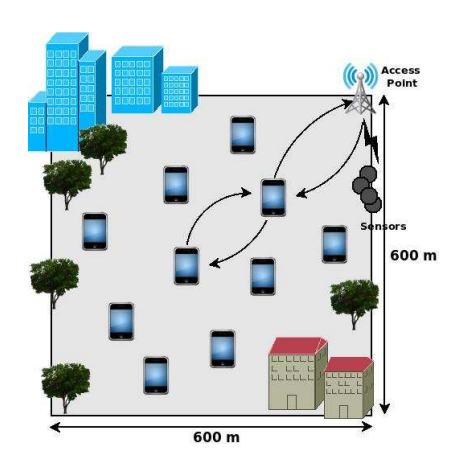
\includegraphics[width=6.5cm]{../fig1.png}
		\end{center}
	}


	%%% Bild 2 %%%%%%%%%%%%%%%%%%%%%%%%%%%%%%%%%%%%%%%%%%%%%%%%%%%%%%%%%%%%%%%%%%%%%
	\headerbox{\textsf{Fig. 2: Results of the first experiment}}{name=bild2,column=4, span=2, below=bild1}{

		\begin{center}
			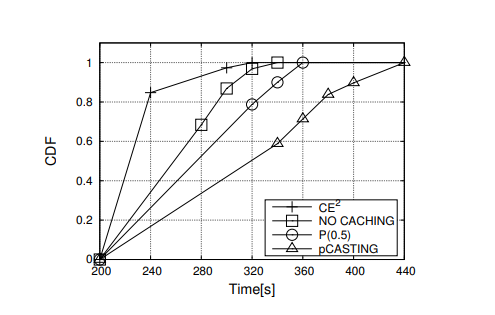
\includegraphics[width=7.5cm]{../fig2.png}
		\end{center}
		\begin{center}
			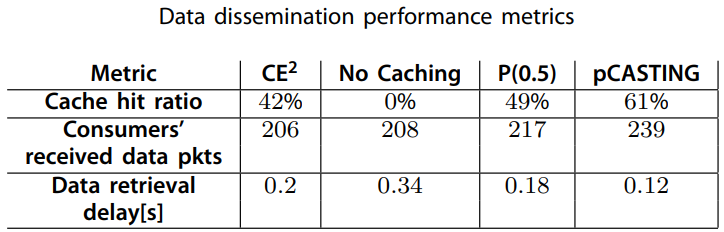
\includegraphics[width=7.5cm]{table2.png}
		\end{center}
	}


	%%% Bild 3 %%%%%%%%%%%%%%%%%%%%%%%%%%%%%%%%%%%%%%%%%%%%%%%%%%%%%%%%%%%%%%%%%%%%%
	\headerbox{\textsf{Fig. 3: Results of the second experiment}}{name=bild3, column=4, span=2, below=bild2, above=bottom}{
		\centering
		\begin{center}
			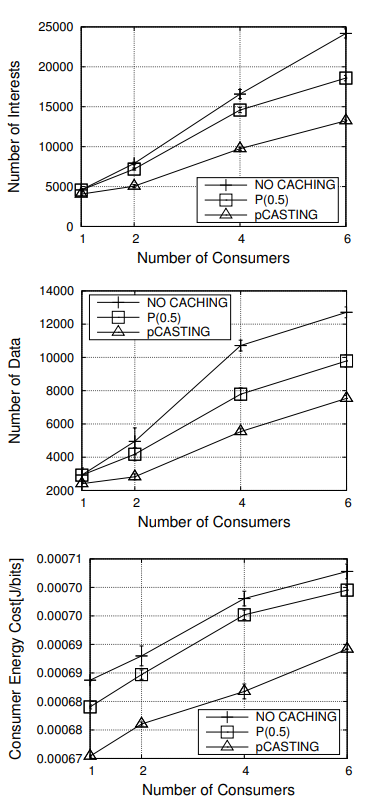
\includegraphics[height=11.5cm]{results2_vertical.png}
		\end{center}
	}


	%%% References %%%%%%%%%%%%%%%%%%%%%%%%%%%%%%%%%%%%%%%%%%%%%%%%%%%%%%%%%%%%%%%%%%%%%
	\headerbox{\textsf{References}}{name=references, column=0, span=4, above=bottom, below=abschnitt4}{
		\begin{small}
			\renewcommand{\refname}{}
			\setlength{\parskip}{0cm}
			\setlength{\bibsep}{0cm}
			\bibliographystyle{unsrt}
			\bibliography{references}
		\end{small}

		\vspace{-0.3cm}
		\renewcommand{\refname}{}
		\begin{thebibliography}{00}
			% \bibitem{b1} J. Gubbi, R. Buyya, S. Marusic, and M. Palaniswami, "Internet of Things (IoT): A Vision, Architectural Elements, and Future Directions," \textit{Elsevier Future Generation Computer Systems}, Volume 29, No. 7, 2013.
			% \bibitem{b2} B. Ahlgren, C. Dannewitz, C. Imbrenda, D. Kutscher, and B. Ohlman, "A Survey of Information-Centric Networking," \textit{IEEE Communications Magazine}, vol. 50, no. 7, pp. 26-36, 2012.
			% \bibitem{b3} Y. Zhang \textit{et al.}, "ICN based Architecture for IoT - Requirements and Challenges," in \textit{Internet-Draft}, 2014.
			% \bibitem{b4} M. Amadeo, C. Campolo, A. Iera, and A. Molinaro, "Named Data Networking for IoT: an Architectural Perspective," in \textit{European Conference on Networks and Communications (EuCNC)}, Bologna, Italy, 2014.
			% \bibitem{b5} G. Zhang, Y. Li, and T. Lin, "Caching in Information Centric Networking: a Survey," \textit{Elsevier Computer Networks}, vol. 57, no. 16, 2013.
			% \bibitem{b6} E. Baccelli et al., "Information Centric Networking in the IoT: Experiments with NDN in the Wild," \textit{ACM ICN}, 2014.
			% \bibitem{b7} J. Quevedo, D. Corujo, and R. Aguiar, "Consumer Driven Information Freshness Approach for Content Centric Networking," in \textit{IEEE INFOCOM NOM Workshop}, 2014.
			% \bibitem{b8} S. Vural et al., "In-network Caching of Internet-of-Things Data," in \textit{IEEE ICC}, 2014.
			\bibitem{b9} L. Zhang et al., "Named Data Networking (NDN) Project," PARC, Tech. Rep. NDN-0001, October 2010.
			% \bibitem{b10} A. Afanasyev et al., "ndnSIM: NDN simulator for NS-3," University of California, Los Angeles, Tech. Rep. NDN-0005, 2012.
			% \bibitem{b11} I. Psaras et al., "Probabilistic In-Network Caching for Information-Centric Networks," in \textit{ACM ICN'12}, 2012.
			% \bibitem{b12} S. Tarnoi, K. Suksomboon, W. Kumwilaisak, and Y. Ji, "Performance of Probabilistic Caching and Cache Replacement Policies for Content-Centric Networks," in \textit{IEEE LCN}, 2014.
			% \bibitem{b13} W. Shang et al., "Securing Building Management Systems Using Named Data Networking," \textit{IEEE Network}, vol. 3, no. 28, 2014.
			% \bibitem{b14} L. Wang et al., "Rapid Traffic Information Dissemination Using Named Data," in \textit{ACM NoM'12}, 2012.
			% \bibitem{b15} M. Amadeo, C. Campolo, and A. Molinaro, "Forwarding Strategies in Named Data Wireless Ad Hoc Networks: Design and Evaluation," \textit{Elsevier Journal of Network and Computer Applications}, 2014.
			% \bibitem{b16} I. Rhee, M. Shin, S. Hong, K. Lee, and S. Chong, "On the Levy-walk Nature of Human Mobility," in \textit{IEEE INFOCOM}, 2008.
			% \bibitem{b17} "Cisco Aironet 802.11a/b/g Wireless Cardbus Adapter, Data Sheet on line at http://www.cisco.com."
			% \bibitem{b18} "The network simulator-3 (ns-3), http://www.nsnam.org/."
		\end{thebibliography}
	}

\end{poster}

\end{document}
